\documentclass{article}
\usepackage{hyperref}
\usepackage{datetime}
\usepackage{listings}
\usepackage{graphicx}
\usepackage{float}

\title{Automated Continious Integration with Travis}
\newdate{date}{24}{02}{2020}
\date{\displaydate{date}}
\author{John Ghatas}

\hypersetup{
    colorlinks=true,
    linkcolor=black,
    urlcolor=red,
    linktoc=all
}

\begin{document}
    % Page 1
    \maketitle
    \newpage
    
    % Page 2
    \tableofcontents
    \newpage

    % Page 3
    \section{Project definition}
    \paragraph{Goal}{This project was pulled from a Lynda tutorial teaching the basics of Docker, 
    the Docker container created runs an express backend using MongoDB as the database server.}

    \subsection{Running the application locally}{The first order of business was to ensure that the application
    was able to run locally before deploying it in a Docker container. To do this we ran the following commands in
    the main directory:
    \begin{lstlisting}[language=bash]
        $ npm install
        $ npm start
    \end{lstlisting}
    To start the backend locally \textbf{MongoDB} is required to have a local install.
    }

    \subsection{Exporting to docker}{The next step was to export the image to docker locally, to ensure the setup was
    running before deploying the automation of the Docker image to the TravisCI servers. To build a Docker image, I had to create
    a Dockerfile specifying the steps that needed to be taken to deploy the Express backend in a Docker container. The Dockerfile
    is shown in \textbf{Figure \ref{fig:dockerfile}}.}
    
    \begin{figure}[H]
        \centering
        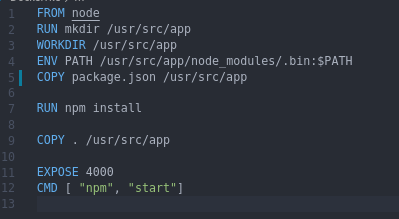
\includegraphics[scale=3, pagebox=artbox]{Images/Dockerfile.png}
        \caption{The dockerfile containing the instructions for building the container}
        \label{fig:dockerfile}
    \end{figure}




\end{document}